\documentclass[fleqn]{article}

\usepackage{geometry}
\usepackage{amsmath, nccmath}
\usepackage{amssymb}
\usepackage{graphicx}
\usepackage{enumitem}
\usepackage[nodisplayskipstretch]{setspace}
\usepackage{float}

\title{Homework 1}
\author{Owen Sowatzke}
\date{September 12, 2023}

\begin{document}

	\setlength{\abovedisplayskip}{0pt}
	\setlength{\belowdisplayskip}{0pt}
	\setlength{\abovedisplayshortskip}{0pt}
	\setlength{\belowdisplayshortskip}{0pt}
	\setlength{\mathindent}{0pt}
	\doublespacing
	\maketitle
	
	\begin{enumerate}[nolistsep]
	
		\item[2.7] Determine whether each of the following signals is periodic. If the signal is periodic, state its period.
		
		\begin{enumerate}[nolistsep]
			
			\item[(b)] $x[n] = e^{j({3\pi}n/4)}$
			
			\begin{align*}
			\frac{\omega}{2\pi} = \frac{k}{N}
			\end{align*}
			
			\begin{align*}
			\frac{3\pi/4}{2\pi} = \frac{k}{N}
			\end{align*}
			
			\begin{align*}
			\frac{3}{8} = \frac{k}{N}
			\end{align*}
			
			Because $\frac{k}{N}$ is rational, the signal is periodic, and the period of the signal is $N = 8$.
			
			\item[(d)] $x[n] = e^{j{\pi}n/\sqrt{2}}$
			
			\begin{align*}
			\frac{\omega}{2\pi} = \frac{k}{N}
			\end{align*}
			
			\begin{align*}
			\frac{\pi/\sqrt{2}}{2\pi} = \frac{k}{N}
			\end{align*}
			
			\begin{align*}
			\frac{1}{2\sqrt{2}} = \frac{k}{N}
			\end{align*}
			
			Because $\frac{k}{N}$ is irrational, the signal is not periodic.
			
		\end{enumerate}
		\item[2.21] A discrete-time signal $x[n]$ is shown in Figure \ref{prob_statement}.
		
		%\renewcommand{\thefigure}{P2.21}	
	
		\begin{figure}[H]		\centerline{\fbox{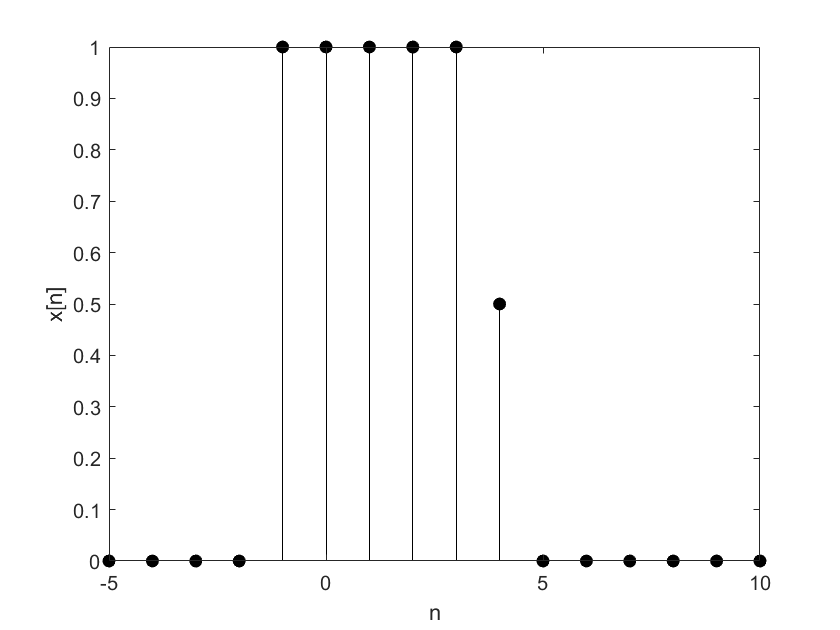
\includegraphics[width=0.35\textwidth]{p2.21_problem_statement.png}}}
		\caption{Discrete Time Signal $x[n]$}
		\label{prob_statement}
		\end{figure}
		
		Sketch and label carefully each of the following signals:
		
		\begin{enumerate}[nolistsep]
			\item[(c)] $x[2n]$
			
			%\renewcommand{\thefigure}{\arabic{figure}}
			%\setcounter{figure}{0}
			
			\begin{figure}[H]				
			\centerline{\fbox{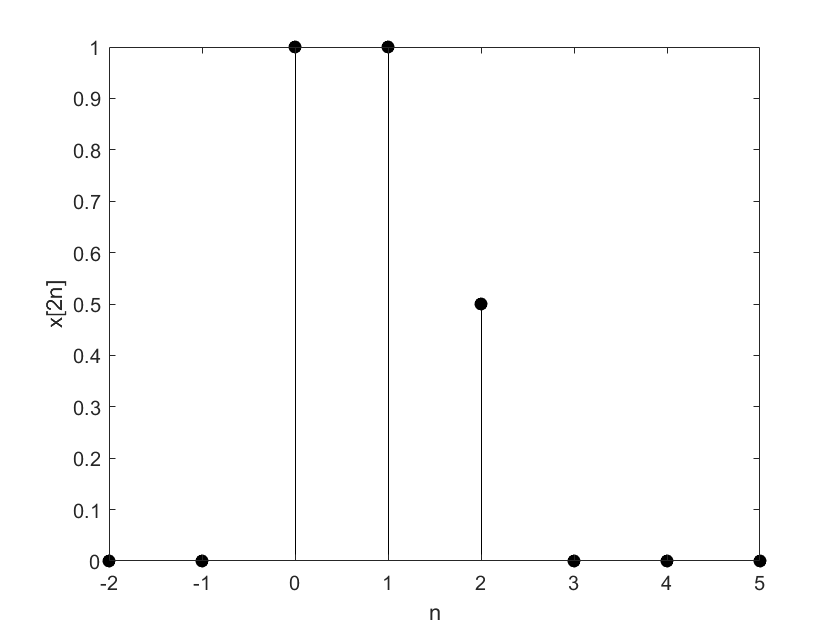
\includegraphics[width=0.35\textwidth]{p2.21_c.png}}}
		\caption{Discrete Time Signal $x[2n]$}
		\label{part_c}
		\end{figure}
		
			\item[(e)] $x[n - 1]\delta[n - 3]$
			
			\begin{figure}[H]
			\centerline{\fbox{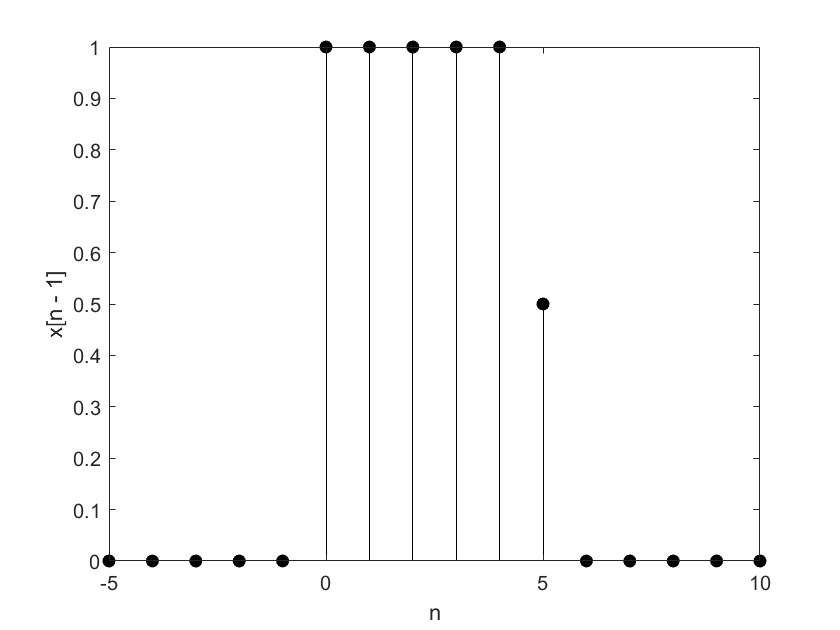
\includegraphics[width=0.35\textwidth]{p2.21_e_x_nm1.png}}}
		\caption{Discrete Time Signal $x[n-1]$}
		\label{part_e_x_nm1}
		\end{figure}
			
			\begin{figure}[H]
			\centerline{\fbox{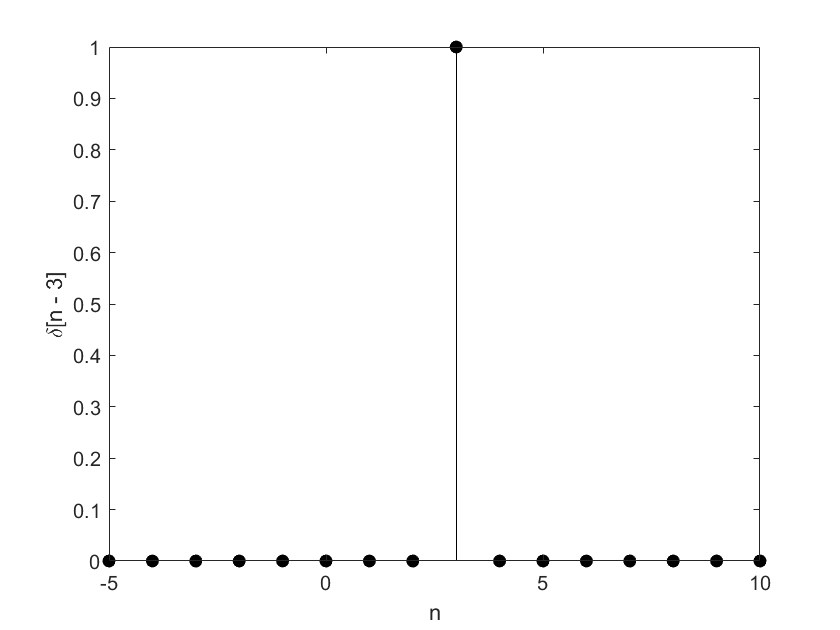
\includegraphics[width=0.35\textwidth]{p2.21_e_delta_nm3.png}}}
		\caption{Discrete Time Signal $\delta[n-3]$}
		\label{part_e_delta_nm3}
		\end{figure}
		
		\begin{figure}[H]
			\centerline{\fbox{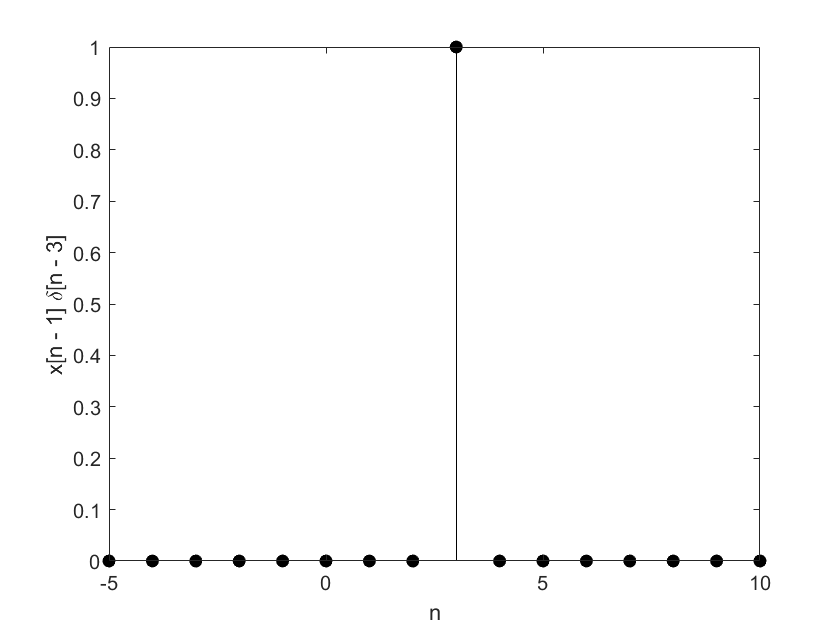
\includegraphics[width=0.35\textwidth]{p2.21_e.png}}}
		\caption{Discrete Time Signal $x[n-1]\delta[n-3]$}
		\label{part_e}
		\end{figure}
		
		\end{enumerate}
		
		\item[2.23] For each of the following systems, determine whether the system is (1) stable, (2) causal, (3) linear, and (4) time invariant.
		
		\begin{enumerate}[nolistsep]
			\item[(a)] $T(x[n]) = (cos{\pi}n)x[n]$
			
				\begin{enumerate}[nolistsep]
				
					\item[(1)] Check whether the system is stable:
			
					Let $y[n] = T(x[n])$
			
					If $|x[n]| \leq B_x\ \forall n$
			
					$|y[n]| = |(cos{\pi}n)x[n]| \leq |cos{\pi}n||x[n]| \leq B_x$
			
					For every bounded $x[n]$ the output $y[n]$ is also bounded.
			
					$\therefore$ the system is stable.
					
					\item[(2)] Check whether the system is causal:
					
					Let $y[n] = T(x[n])$
					
					The output $y[n]$ does not depend on future values of $x[n]$.
					
					$\therefore$ the system is causal.
					
					\item[(3)] Check whether the system is linear:
					
					Let $y_1[n] = T(x_1[n])$ and $y_2[n] = T(x_2[n])$
					
					$T(ax_1[n] + bx_2[n])$
					
					$ = (cos{\pi}n)(ax_1[n] + bx_2[n])$
					
					$ = a(cos{\pi}n)x_1[n] + b(cos{\pi}n)x_2[n]$
					
					$ = ay_1[n] + by_2[n]$
					
					Because $T(ax_1[n] + bx_2[n]) = ay_1[n] + by_2[n]$, the system is linear.
					
					\item[(4)] Check whether the system is time invariant:
					
					$T(x[n-n_0]) = (cos{\pi}n)x[n-n_0]$
					
					$y[n-n_0] = (cos{\pi}(n-n_0))x[n-n_0]$
					
					Because $y[n-n_0] \neq T(x[n-n_0])$, the system is not time invariant.
				\end{enumerate}
					
				\item[(c)] $T(x[n]) = x[n]\sum_{k=0}^{\infty}{\delta[n-k]} = x[n]u[n]$
					
				\begin{enumerate}[nolistsep]
					\item[(1)] Check whether the system is stable:
			
					Let $y[n] = T(x[n])$
			
					If $|x[n]| \leq B_x\ \forall n$
			
					$|y[n]| = |x[n]u[n]| \leq |x[n]| \leq B_x$
			
					For every bounded $x[n]$ the output $y[n]$ is also bounded.
			
					$\therefore$ the system is stable.
					
					\item[(2)] Check whether the system is causal:
					
					Let $y[n] = T(x[n])$
					
					The output $y[n]$ does not depend on future values of $x[n]$.
					
					$\therefore$ the system is causal.
					
					\item[(3)] Check whether the system is linear:
					
					Let $y_1[n] = T(x_1[n])$ and $y_2[n] = T(x_2[n])$
					
					$T(ax_1[n] + bx_2[n])$
					
					$ = (ax_1[n] + bx_2[n])u[n]$
					
					$ = ax_1[n]u[n] + bx_2[n]u[n]$
					
					$ = ay_1[n] + by_2[n]$
					
					Because $T(ax_1[n] + bx_2[n]) = ay_1[n] + by_2[n]$, the system is linear.
					
					\item[(4)] Check whether the system is time invariant:
					
					$T(x[n-n_0]) = x[n-n_0]u[n]$
					
					$y[n-n_0] = x[n-n_0]u[n-n_0]$
					
					Because $y[n-n_0] \neq T(x[n-n_0])$, the system is not time invariant.
				\end{enumerate}
			
			
			
		\end{enumerate}
		
		\item[2.28] Four input-output pairs of a particular system $S$ are specified in Figure P.28-1
		
			\begin{enumerate}
				\item[(c)] Suppose (2) and (3) are input-output pairs of a particular system $S_2$, and the system is known to be LTI. What is $h[n]$, the impulse response of the system?
				
				Let $x_1[n]$ and $y_1[n]$ be the input-output pairs defined by (2), and let $x_2[n]$ and $y_2[n]$ be the input-output pairs define by (3).
				
			$x_1[n] = \delta[n] + \delta[n-2]$
			
			$y_1[n] = \delta[n-1] + 2\delta[n-3] + \delta[n-5]$
			
			$x_2[n] = \delta[n-1] + \delta[n-2]$
			
			$y_2[n] = \delta[n-2] + \delta[n-3] + \delta[n-4] + \delta[n-5]$
			
			We can form $\delta[n]$ using a sum of scaled and delayed copies of $x_1[n]$ and $x_2[n]$. Since $S_2$ is LTI, the impulse response $h[n]$ can be computed using the same sum of scaled and delayed copies of $y_1[n]$ and $y_2[n]$.
			
			$x_2[n+1] - x_2[n]$
			
			$ = (\delta[n] + \delta[n-1]) - (\delta[n-1] + \delta[n-2])$
			
			$ = \delta[n] + \delta[n-1] - \delta[n-1] - \delta[n-2]$
			
			$ = \delta[n] - \delta[n-2]$
			
			$x_1[n] + x_2[n+1] - x_2[n]$
			
			$ = \delta[n] + \delta[n-2] + \delta[n] - \delta[n-2]$
			
			$ = 2\delta[n]$
			
			$\Rightarrow \delta[n] = \frac{1}{2}(x_1[n] + x_2[n+1] - x_2[n])$
			
			$h[n] = T(\delta[n])$
			
			$ = T(\frac{1}{2}(x_1[n] + x_2[n+1] - x_2[n]))$
			
			$ = \frac{1}{2}T(x_1[n] + x_2[n+1] - x_2[n])$
			
			$ = \frac{1}{2}(y_1[n] + y_2[n+1] - y_2[n])$
			
			$ = \frac{1}{2}\{\delta[n-1] + 2\delta[n-3] + \delta[n-5]$
			
			$ + \delta[n-1] + \delta[n-2] + \delta[n-3] + \delta[n-4]$
			
			$ - (\delta[n-2] + \delta[n-3] + \delta[n-4] + \delta[n-5])\}$
			
			$ = \frac{1}{2}(\delta[n-1] + 2\delta[n-3] + \delta[n-5] + \delta[n-1] - \delta[n-5])$
			
			$ = \frac{1}{2}(2\delta[n-1] + 2\delta[n-3])$
			
			$ = \delta[n-1] + \delta[n-3]$
			\end{enumerate}
		
	\end{enumerate}
\end{document}